\documentclass[tikz, border=3mm]{standalone}
\usepackage{tikz}
\usetikzlibrary{arrows.meta, decorations.markings, angles, quotes, positioning}

\begin{document}
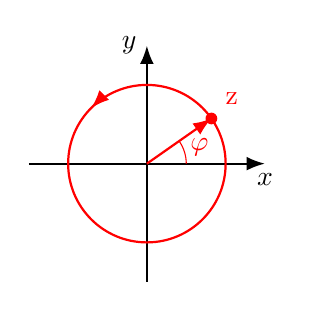
\begin{tikzpicture}[
    >=Latex, % Set default arrow tip style
    path/.style={red, thick}, % Style for the path and vector
    dot/.style={fill=red, circle, inner sep=1.5pt}, % Style for point z
    labelstyle/.style={red} % Style for labels
]

    % Axes
    \draw[->, thick] (-1.5, 0) -- (1.5, 0) node[below] {$x$};
    \draw[->, thick] (0, -1.5) -- (0, 1.5) node[left] {$y$};

    % Define origin, radius, and angle for z
    \coordinate (O) at (0,0);
    \def\radius{1.0} % Radius of the circle
    \def\zangle{35}  % Angle for point z in degrees

    % Calculate point z using polar coordinates
    \coordinate (z) at (\zangle:\radius);

    % Draw the red circle with counter-clockwise arrow
    \draw[path,
        postaction={decorate, decoration={markings, mark=at position 0.375 with {\arrow{>}}}} % Arrow near top-left (135 deg = 0.375)
    ] (O) circle (\radius);

    % Draw point z indicator and label
    \node[dot, label={[labelstyle]above right:z}] at (z) {};

    % Draw vector from origin to z
    \draw[path, ->] (O) -- (z);

    % Draw angle phi
    \coordinate (xaxis_ref) at (\radius,0); % Reference point on positive x-axis
    \pic [draw, labelstyle, angle radius=0.5cm, "$\varphi$", angle eccentricity=1.4] {angle = xaxis_ref--O--z};

\end{tikzpicture}
\end{document}